\documentclass[5p,twocolumn,10pt,times]{elsarticle}
\usepackage{amsmath}
\usepackage{hyperref} % added [draft] to avoid compilation issues that happen if a link is split and appears in two pages
%\modulolinenumbers[5]
\addtolength{\textheight}{8mm}
\addtolength{\textwidth}{4mm}
\addtolength{\voffset}{-10mm}
\addtolength{\hoffset}{-3mm}

\bibliographystyle{elsarticle-num-names}


% ACM template
%
%\documentclass[acmtog,anonymous,timestamp,review]{acmart}
%
%\usepackage{booktabs} % For formal tables
%




% My TK added packages and commands

	% for for using hyperref and elsarticle-num-names together in order to get \citeauthor to work
	\makeatletter
	\providecommand{\doi}[1]{%
	  \begingroup
	    \let\bibinfo\@secondoftwo
	    \urlstyle{rm}%
	    \href{http://dx.doi.org/#1}{%
	      doi:\discretionary{}{}{}%
	      \nolinkurl{#1}%
	    }%
	  \endgroup
	}
	\makeatother

	% have multiline subfigure captions be centered
	\usepackage[labelformat=parens]{subcaption} % subfigures
	\captionsetup[subfigure]{justification=centering}
	\captionsetup{subrefformat=parens} % pure refernce subfigure with parentheses: fig.10a and (b)
	%\renewcommand\thesubfigure{(\alph{subfigure})} % refernce subfigure always with parentheses: fig.10(a) and (b)

	\captionsetup[figure]{labelfont={bf},name={Fig.},labelsep=period} % use `Fig.' for figure subscript instead of `Figure'
	
	\usepackage[export]{adjustbox} % [right] alignment for includegraphics
	
	\usepackage{rotating} % turn env for rotating text in figures

	\usepackage{wrapfig} % inline figures

	% tables
	\usepackage{multirow} % multicolumn, multirow
	\usepackage{colortbl} % \cellcolor{<color>}
	\newcolumntype{C}[1]{>{\centering\arraybackslash}m{#1}}   %% centered
	\newcolumntype{R}[1]{>{\raggedleft\arraybackslash}m{#1}}  %% right aligned

	\usepackage[capitalise]{cleveref} % automatically add `Fig.'  etc before a reference.

        \usepackage{ amssymb } % \therefore
	
	\newcommand{\degree}{^\circ}
	
	\usepackage[binary-units]{siunitx} % mm and stuff
	\sisetup{per-mode = symbol}
	\DeclareSIUnit\pixel{px}

	\usepackage{units} % \nicefrac{3}{8}
	
	
	
	\DeclareMathOperator*{\argmax}{arg\,max}
	\DeclareMathOperator*{\argmin}{arg\,min}
	
	\DeclareMathOperator{\abs}{abs} % absolute function

	\usepackage{amsthm} % \begin{proof}
	\newtheorem{lemma}{Lemma}[section]
	\theoremstyle{definition}
	\newtheorem{definition}{Definition}[section]

	\usepackage[inline]{enumitem} % inline enumerate*

	\usepackage[toc,page]{appendix} % appendicces
	
	\usepackage{pgfplots}
	\usepackage{pgfplotstable} % tikzpicture table plots
	\pgfplotsset{compat=1.15}
	\usetikzlibrary{backgrounds}

	\usepackage[noend]{algpseudocode} % algorithmic
	\usepackage{algorithm} % wrapper for pseudocode to give a caption and label

	\newcommand{\pluseq}{\mathrel{+}=} %pluseq symbol
	\usepackage{upgreek} % \uplambda

	\usepackage{listings} % for listing C++ code instead of pseudocode
	\lstset{ 
      breaklines=true,                 % sets automatic line breaking
      basicstyle=\ttfamily,
      mathescape
    }




    % \usepackage[disable]{todonotes} % notes not showed  
    % \usepackage[draft]{todonotes}   % notes showed
    \usepackage{color,soul} % caps, highlight (\hl)

	\newcommand{\comment}[1]{}
	
%    \newcommand{\todo}[1]{\hl{#1}}
%    
%	\newcommand{\temp}[1]{\textcolor[rgb]{0, 0, 0.2}{#1}}
%	\newcommand{\tim}[1]{\temp{\todo{[Tim: #1]}}}
%	\newcommand{\jun}[1]{\temp{\todo{[Jun: #1]}}}
%	
%	\newcommand{\old}[1]{\textcolor{gray}{#1}}
	\usepackage[normalem]{ulem}
	\newcommand{\stkout}[1]{\ifmmode\text{\sout{\ensuremath{#1}}}\else\sout{#1}\fi}
	
	% Revise macro (usage: \revise{old}{new})
	% Version a) First arg red and striked out, second argument green
	\newcommand{\revise}[2]{\noindent{\color{red}{\stkout{#1}}}\noindent{\color{blue}{#2}}}
	% Version b) First arg ignored, second argument green
	%\newcommand{\revise}[2]{\textcolor{blue}{#2}}
	% Version c) First arg ignored, second argument unchanged (for final draft)
	%\newcommand{\revise}[2]{#2}

	\usepackage{alltt}
	
	\newcommand{\question}[1]{{\bf#1}}
	\newcommand{\todo}[1]{\par\noindent{\bf \color{orange}#1}}
	\newcommand{\commits}[1]{{\bf\begin{alltt} {#1}\end{alltt}}}
	\renewcommand{\commits}[1]{}
	\newcommand{\response}[1]{{#1}}
\newcommand\paper[2]{\par changes to \emph{#1} --- ``#2'' }
\renewcommand\paper[2]{\par changes to \emph{#1} --- ``\dots'' }

\newcommand\Que[1]{%
   \leavevmode\par
   \stepcounter{question}
   \noindent
   \thequestion. {\bf#1}\par}

\newcounter{question}
\setcounter{question}{0}

\numberwithin{question}{section}


\usepackage{chngcntr}

\newcommand\subQue[1]{%
   \leavevmode\par
   \stepcounter{subquestion}
   \noindent
   \thesubquestion. {\bf#1}\par}

\newcounter{subquestion}
\setcounter{subquestion}{0}

\counterwithin{subquestion}{question}


\newcommand\Ans[2][]{%
    \leavevmode\par\noindent
   {%\leftskip37pt
    {\it Response:} \textbf{#1}#2\par}}



	\setulcolor{red}

	\usepackage[normalem]{ulem} % squigly underline

	\renewcommand\floatpagefraction{.8}



	\newlength{\figwidth}
	\newlength{\figwidthTwo}
	\newlength{\figwidthTree}
	\newlength{\figheight}
	\newlength{\figheightTwo}
	\newlength{\tempheight}
	\newlength{\tempheightTwo}

	% deal with missing images which are not directly included in the repo
	\iffalse
	\newcommand{\noimage}[1]{%
	  \setlength{\fboxsep}{-\fboxrule}%
	  \fbox{\phantom{\rule{10pt}{10pt}} Missing file: \path{#1} \phantom{\rule{10pt}{10pt}}}% Framed box
	}
	\let\includegraphicsoriginal\includegraphics
	\renewcommand{\includegraphics}[2][width=\textwidth]{\IfFileExists{#2}{\includegraphicsoriginal[#1]{#2}}{\noimage{#2}}}

	\fi
% ENd of TK's added packages and commands



\begin{document}
\baselineskip11pt 

\begin{frontmatter} 

\title{
Response to reviewers
\\
\large{A framework for adaptive width control of dense contour-parallel toolpaths in \revise{additive manufacturing}{fused deposition modeling}}
}


%\author{Paper ID: xxx}

\author[um,tud]{Tim Kuipers}
\author[tud]{Eugeni L. Doubrovski}
\author[tud]{Jun Wu}
\author[cuhk]{Charlie Wang}
% \ead{cwang@mae.cuhk.edu.hk}
\address[um]{Ultimaker, Utrecht, The Netherlands}
\address[tud]{Department of Design Engineering, Delft University of Technology, The Netherlands}
\address[cuhk]{Department of Mechanical and Automation Engineering, The Chinese University of Hong Kong, Hong Kong SAR, China}

\begin{abstract}
We have more clearly distinguished our work from existing methods.
We have introduced extensions to the beading schemes:
\begin{enumerate*}
\item the widening meta-scheme is extended with a minimal feature size, in order to allow for a fair comparison between the various techniques 
and
\item a limiting meta-scheme is introduced which only generates the outer $N$ insets, so that the framework can readily be combined with the direction-parallel strategy in a manner common in FDM.
\end{enumerate*}
The results have been recalculated accordingly.
We have developed a new manufacturing method which doesn't rely on custom machinery and which clearly shows the feasibility of adaptive bead width.
We have computed fabrication time results.
We have added a video animation explaining the union of cones approach in an intuitive manner.
We have made various language fixes and improvements to images to address some of the reviewers' comments.
\end{abstract}

%
% The code below should be generated by the tool at
% http://dl.acm.org/ccs.cfm
% Please copy and paste the code instead of the example below.
%
%\begin{CCSXML}
%\end{CCSXML}

%\ccsdesc[500]{Computer systems organization~Embedded systems}
%\ccsdesc[300]{Computer systems organization~Redundancy}
%\ccsdesc{Computer systems organization~Robotics}
%\ccsdesc[100]{Networks~Network reliability}

\end{frontmatter}

We are very grateful for the feedback and contributions of the reviewers.
We feel that their feedback has provoked a leap forward in quality of the presented manuscript.







\Que{Example question by reviewer}
\Ans{Example response}
\revise{Old text in manuscript}{New text in manuscript}
\todo{Comment for us internally (should be removed before this letter is sent).}
\commits{123commit-hash}

\section{Reviewer 1}
Overall, the paper proposes some novel frameworks which are meaningful to additive manufacturing. Therefore, I suggest it for publication once the following major comments are addressed. 





%\stepcounter{question}
\Que{
Could the authors provide a mathematical foundation for the relationship between the underfill/overfill areas and the allowed variation of bead width?
I believe the proposed beading scheme can reduce the underfill/overfill areas somehow.
But we still lack a mathematical theory to guide the design.
}
\Ans{
The relationship between under-/overfill and bead widths can be split into several components:
\begin{enumerate*}
\item depending on the feature size
\item depending on the change in feature size
\item depending on the topology
\end{enumerate*}
.
In the first case we consider a part with a constant feature size, in the second we consider the rate of change of feature size and in the thirs we consider the influence of 3-way intersections.

1. When considering a part with constant feature diameter $d$ we note that the beading only depends on the feature diameter: $B(n, r) = B(q(2r), r)$.
From the beading function we can easily derive the under-/overfill by summing over the bead widths $W$.
We can then derive that the naive scheme produces over-/underfill at all diameters except $d=2i w^*$, the center scheme for $(i + 0.8) w^* < d < (i+ 1.25) w^*$ and the constant and distributed schemes nowhere (except for features smaller than $w^*$).
We have added a paragraph to the new section 5.1 Theoretical consideration to explain this and the implications for design for additive manufacturing.

2. When the feature size changes the amount of over-/underfill is related to a bisector angle $\alpha < \alpha_\text{max}$ according to the formula already given in section 3.3, paragraph `Significance measure': 
``This corresponds to overfill areas and underfill areas the size of $\nicefrac12 (w^*)^2 \left( \nicefrac14 \tan ( \alpha / 2) - \alpha / 2 \right)$''.
This formula is also relevant for the other beading schemes because the nonsignificant regions are filled in a similar fashion to the naive technique.
For small bisector angles these under-/overfill areas are considered to be permittably small.
We hope that this explanation suffices for the reviewer and the existing text suffices for the general reader.

3. The topology also has an influence on underfill. For example, a 3-way intersection in a 3D model which is a honeycomb pattern with a feature diameter of $w^*$ causes some over and underfill using \emph{any} possible technique, because 3 printed beads come together in the same point.
Also a honeycomb of $2w^*$ diameter causes some underfill in the center;
when 3 beads surround a single point there will always remain a micro-gap because of the high viscosity of the molten filament.
This is handled in Fig. 12 and the last paragraph of section 3.6.

As for `the allowed variation of bead width': our vision \emph{was} that there should be no binary criterion for manufacturability and instead there should only be a floating number evaluation of manufacturability of a given bead width.
However, we have now put bounds on the induced bead widths, so that the reader could compare our method to any range of `allowed variation' according to any manufacturability criterion.
See the answer to question 3.4.
}

\commits{2e1c40be93f92a8495c0d7fa379e983dd3ee7b98
3b13960e15c07f484ab641a2d941f6086eda571c
5b8c5971d606089754ba118560e51ec6d7dfda0b % new section
}
\paper{Conclusion}{
\revise{}{It is expected that as distributed beading schemes are implemented in commercial software packages and bead width variation control become commonplace, the practice of design for additive manufacturing can disregards most of the nozzle size considerations.}
}

\stepcounter{question}





\subQue{
The authors should highlight their contributions compared to the existing approaches for generating toolpaths with adaptive width.
}
\Ans{
See also our response to 1.5.
}
\todo{
Describe changes
}
\commits{66d006d91d406c0064ee1f4f1e4df85fc0821994 e806d40e5e6d2bbe450c6792b802f0fcce4df645}
\paper{Intro}{
 \begin{itemize}
\item A geometric framework \revise{for generating densely filling contour-parallel toolpaths employing adaptive width, according to any beading scheme which decides on the bead spacing and widths.}{allowing various adaptive bead width control schemes used to generate contour-parallel toolpaths which minimize under- and overfill.}
\item A specific beading scheme for FDM printing which \revise{}{furthermore} reduces the amount of deviation in the extrusion widths compared to existing literature, and which \revise{promotes smooth toolpaths that are equal to the preferred width toward the outline of the shape.}{produces beads of exactly the preferred width outside of central regions of the outline shape.}
 \end{itemize}}
 \paper{intro}{In this paper we propose a framework for planning toolpaths with control over the adaptive width \revise{for}{while} minimizing over- and underfill.}





\subQue{
From Fig. 1(b) and (c), we can see that the approach in Jin et al (2017) can fill the sharp right end, but the proposed approach can not. 
}
\Ans{
We now use the same minimal feature size in all approaches.
We have added this functionality to the \emph{widening} meta-scheme.
We have also added a figure to show that functionality.
}
\todo{
Redo the tests with homogeneous $r_\text{min}$

note value of $r_\text{min}$ in paper
}
\commits{
%a5ddf3a73e3df20e43f25eafb93e9ce3a1393b13 
d3fe6c86ee887da0e33fefdc43a83d014bc6047b 
0ac1c930a7cd2d1d305da730c9d5db20f4a8ea3f 
9281d8ae7350539102be0ead7b2ffc611591d2b4 
a88ccd3309aef1233ed00ce9f22b244fe64668f4
}
\paper{Beading schemes}{
\paragraph{Widening \revise{}{meta-scheme}}
Complementary to any of these schemes we can enforce a minimum feature size at no extra cost in our framework.
Regions where the model is narrower than \revise{the nozzle size}{some $r_\text{min}$} can be printed with a bead width \revise{}{$w_\text{min}$} larger than the model thickness.
We can simply override
\begin{align*}
q'(d) &= 
\begin{cases}
0 & \text{ if } 0 \leq d < 2 r_\text{min} \\
1 & \text{ if }  2 r_\text{min} \leq d < w^*  \\
q(d) & \text{ otherwise}
\end{cases}
\\
\revise{}{
W'(n,r)_0} &=
\begin{cases}
\max \left( w_\text{min}  ,  2 r \right) & \text{ if } 2 r < w^* \\
W(n,r)_0 & \text{ otherwise}
\end{cases}
\end{align*}

\revise{}{
\paragraph{Shell meta-scheme}
The industry standard of FDM is to generate only a limited contour-parallel perimeters and to fill the remainder using a direction-parallel strategy.
We therefore provide a meta-scheme to generate adaptive bead width toolpaths only in narrow regions and generate the limited number of perimeters $M$ using the preferred width in regions which are wide enough.
We also take care not to leave gaps which are too small to be filled using the direction-parallel strategy:

\begin{align*}
q'(d) &= \min(M, q(d))
\\
W'(n,r)_i &= 
\begin{cases}
W(n, M w^*)_i & \text{ if } 2 r > q^{-1}(M) \\
W(n,r)_i & \text{ otherwise}
\end{cases}
\end{align*}

These meta-schemes introduce non-linearities in the quantization function.
Because the beading is only evaluated at nodes in the skeleton, we need to make sure that there are nodes at the locations along the skeleton where the non-linearities happen.
We therefore insert extra nodes along with their ribs at locations $v$ with a radial distance $R(v) = r_\text{min}$ for widening and at $R(v) \in \left\{ M w^*, q^{-1}(M), q^{-1}(M) + \nicefrac12 w^* \right\} $ for the transition from narrow shell to unconstrained shell.
Combining all meta-schemes functionality we can generate results such as depicted in \cref{widening_shell}.

\begin{figure}
\centering
\includegraphics[rotate=90,width=.6\columnwidth]{sources-validation-gMat_example_all_combined.png}
\caption{
Toolpath generated with the inward distributed strategy ($N=1.5$) in conjunction with the widening meta-scheme ($W_\text{min}=0.5, 2r_\text{min}=0.2$, see top left) and the shell meta-scheme ($M=4$, see middle).
% -p test_geometry/gMAT_example.svg -b 4 -s i -n 1.5 -a --mins 0.2 --minw .5
Widening and shell require extra edges (green) at key locations in the skeleton.
The azure area is to be filled using some direction-parallel toolpath generation algorithm.
}
\label{widening_shell}
\end{figure}
}

}





\subQue{
If there is no sharp corners exist, then the existing approaches such as Jin et al (2017) do not have to use bead widths of large variations. 
}
\Ans{
The wedge shape of Fig. 1 was chosen because it contains a wide range of feature sizes and is therefore representative for a wide range of models.
Nearly every model induces the full range of $[0.5w^*,1.8w^*]$ using the centered approach by Jin et. al. 2017 JMS,
because nearly all models have feature sizes which span any range $[iw^*,(i+1)w^*]$ for $i\in\mathcal{N}$.
See Fig. 17 in the paper of Jin et al for an example shape.
Only shapes without central regions (a circle) or shapes with central regions with an exact multiple of $w^*$ everywhere (a rectangle) don't require any variation in bead width, but that holds for any of the beading schemes.

Figure~\ref{no_corners} shows an example of a shape without sharp corners, and which also requires a large bead width variation when using the constant bead count approach by Ding et al.
}
\begin{figure} \centering
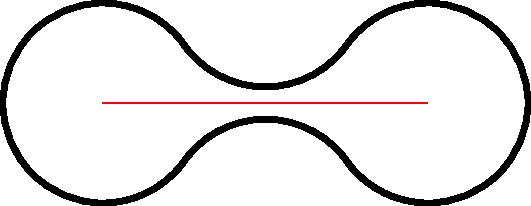
\includegraphics[width=.5\linewidth]{response_no_corners}
\caption{Example shape without sharp corners but with a large variation in feature size.}
\label{no_corners}
\end{figure}





\Que{
How do the authors conduct path planning? Could the authors add a simple 2D geometry with multiple holes to explain the path planning process? As the proposed approach adds more disconnected toolpaths to minimize underfill areas, an improper path planning would significantly increase the fabrication time. 
}

\todo{
Show results on printing time

Mention that the path order is not optimized
}





\Que{
While the proposed approach can use adaptive bead width to minimize underfill and overfill areas, the generated toolpaths are disconnected compared to the traditional approaches. From my experience, a small overfill area does not have to lead to serious defects. But the disconnected filaments definitely have worse mechanical performances compared to the continuous ones. 
}
\Ans{
That is a difficult question.
It might very well be true that discontinuous extrusion lines form a bigger problem than some over- or underfill areas - at least certainly for flexible filaments on a Bowden printer.
However, it is quite hard to find a mathematical approach to balance discontinuity with the size of over-/underfill areas.

It should be noted that even small underfill areas can be unfillable using an overextrusion approach.
For example the microgaps at 3-way intersections.
The viscocity if molten filament is too high to reach into those small crevices.
}
\todo{
count number of extrusion toolpaths?

mention as future work?

That might be true, but the microgaps near 3-way intersections are not fillable using overfilling; the plastic cannot creap into those cravices.
}






\Que{
Why the authors state the inward distributed beading scheme as new? Jin et al (2017) has proposed the strategy to add a toolpath with varying width along the center edges of the skeleton, and with unchanging width outside.
}
\Ans{
The difference between the inward distributed beading scheme and the method by Jin et al 2017 JMS is already shown in Fig 1.b and c. 
It is also shown in Fig. 16 c and e.
In order to clearly address the difference early on we mention the difference in the description of Jin in the introduction.
}
\commits{b7c4d299a76e9fab6c233d572f3248c1350a2e8c}
\paper{Intro}{
\revise{
 Therefore, a narrower range of widths is desirable.
}
{We therefore reduce the bead width range by distributing the workload from the centermost bead over neighboring beads.}
}




\Que{
\label{fig1geometry}
In Fig.1, how to justify the proposed approach as different geometries are used? I believe if the authors use the same geometries as in Fig 1. (a) and (b), there would be also underfill areas using the proposed approach. 
}
\Ans{
There are two ways in which we can interpret this question, leading to two responses.
The question can be interpreted as saying that Fig a has a different geometry than b or c.
There is now a black outline to show that the shapes in Fig 1a, b and c are actually the same geometry, and the output is less confusing because we now use the same minimum feature size for b and c.

The question can also be interpreted as saying that one might use a different shape than the geometry in Fig 1.
We decided on this wedge shape because it shows how the techniques deal with a wide range of feature sizes;
the wedge shape can be read as a graph where we can read out the resulting beading for any local feature size.
}
\commits{45853e8b30d93f60e9465cbb649e347f9cfc23b1 53224c04ceff6c1b18a9eea6de8e7e33957b7797}
\paper{Intro}{
Illustration of different toolpath\revise{}{s} for a \revise{wedge }{}shape \revise{}{showcasing a range of shape radii }\revise{}{(black)}.
}
\paper{Intro wedge figure}{
\revise{}{These results can be read as a graph with feature size on the horizontal axis and its corresponding beading along the vertical axis.}
}



\Que{
Please double check the following sentences. ”Third, the extruded path should ...”(at the second paragraph of Section 2) ”This the downward phase...” (at the last paragraph of Section 3.5) 
}
\Ans{
Okay. Thanks.
}
\commits{eb2a5207c83dfe069d3ab3fc37bf2149b8a51964}
\paper{Related work}{
Third, the extruded path should cover \revise{a }{}the region of the contour without gaps.
}
\paper{Related work}{
\revise{This the}{The} downward phase makes sure that all nodes have a beading associated with it, so that the slicing algorithm can efficiently slice the edges leading up to a marked or unmarked node.  
}






\Que{
In Fig.4, the bead count should marked in another way. The ultra thick solid line conflicts with that for ”outline”. 
}
\Ans{
Note that the bead count is the number, not the arrow from the number.
The arrow is now a double thin line.
}
\commits{07df258c1fa618808ba9493384550021a03c83e1}
\paper{Fig 4}
{
See \cref{legend}.
\begin{figure}\centering
\includegraphics[width=.75\columnwidth]{sources-method-legend2.pdf}
\caption{Illustrative explanation of terms and color coding that are consistently used in this paper.}
\label{legend}
\end{figure}
}




\Que{
What are the differences between the distributed and the inward scheme in Fig. 16(d) and (e)? Are they the same? 
}
\Ans{
We have adjusted the range of the inward distributed scheme to $N=2$ in order to generate a bigger difference between these images.
}
\commits{735762b1e7daf31ae4465bf288ef867ded7da095 93352058a46fb391e323df16f45466adb8cad508}
\paper{Beading schemes}
{
See \cref{distributed_comparison}.
\begin{figure}
\centering
\setlength{\figwidth}{.8\columnwidth}
\setlength{\figheight}{.3\columnwidth}
\begin{minipage}[b]{0.8\linewidth}
% -p test_geometry/wedge.svg -o wedge -s nrdi -n 1.5 -a --scale 1.5
\begin{subfigure}[t]{\figwidth}\centering
\includegraphics[width=\figwidth]{sources-validation-wedge-Distributed-pretty-evenly.png}
\caption{Evenly distributed}
\end{subfigure}
\begin{subfigure}[t]{\figwidth}\centering
\includegraphics[width=\figwidth]{sources-validation-wedge-Distributed-pretty-inward.png}
\caption{Inward distributed}
\end{subfigure}
\end{minipage}
\begin{subfigure}[t]{.1\columnwidth}\centering
\includegraphics[height=\figheight]{sources-validation-widths-legend-small.pdf}
\end{subfigure}
\caption{
Closeup of toolpaths generated with the distributed \revise{}{and inward ($N=1.5$)} beading schemes for a large wedge shape.
Colors represent bead widths.
}
\label{distributed_comparison}
\end{figure}
}





\Que{
In Fig. 17(b), where is the curve for the ”uniform” case?
}
\Ans{
We've added it back in.
Note that the width of the uniform case is \SI{0.4}{\milli\meter} \emph{everywhere}, so the curve is not really informative.
}
\commits{e5f3649455c73c8146e8d07cce13bc1e89d84cbb}



























\section{Reviewer 2}
The paper is generally well written with clear illustrations. 




\Que{
There are occasional omissions, perhaps unintentional, such as the definition of a skeleton - see section 3.1, second paragraph. 
}
\Ans{
Indeed we have intentionally not defined the term `skeleton'.
It seems that there is no generally accepted \emph{intuitive} definition of `skeleton';
the first occurance of the term was as synonymous with the medial axis and it was only defined \emph{mathematically}.
However, the term is now used as an umbrella term for the various different types of skeleton.
We have changes the wording a bit to make clear that `skeleton' refers to an undefined umbrella term.
}
\commits{5356492b5a9a690228ffdb6a6a26cf10d099a7d4}
\paper{Method overview}{
Our method starts with computing \revise{the}{a type of} skeleton of the input polygon based on the medial axis transform (MAT), a strategy that has been commonly used for generating contour-parallel toolpaths~\cite{eiamsa2003toward}. 
}





\stepcounter{question}
\subQue{
The authors seem to use linear approximations of the medial axis - see Figure 2 (b), which is understandable given the fact that they compute the MA with the Boost library. If this is so, can the authors comment on the implications of this approximation?
}
\Ans{
We chose for linear approximations because they simplify the process,
whereas we chose for Boost because it seemed more stable than alternative libraries.

The discretization is handled in section 3.2. Skeletal trapezoidation, second paragraph.
The discretization simplifies the algorithm, potentially at a slight computational cost.
Because we used $d^\text{discretization} = \SI{0.2}{\milli\meter}$, we can expect the discretized skeleton to deviate from the real skeleton by approximately \SI{0.013}{\milli\meter}, which is within the range of accuracy of the hardware system used.
The computation of this value is complicated by the fact that the discretization always introduces a sample point at the apex and at the boundaries of significant portions of the parabola.
(See section 3.3 Significance measure, last paragraph.)
See Figure~\ref{response_parabola_discretization}.

We don't feel this type of discretization error is worth extending the manuscript with.

\begin{figure}\centering
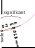
\includegraphics[width=.3\linewidth]{response_parabola_discretization}
\caption{Parabola discretization.
Thick black is part of the outline.
Red is significant skeleton, violet is non-significant skeleton.
}\label{response_parabola_discretization}
\end{figure}
}




\subQue{
For example, what happens if the obtuse outside angle in Figure 2 goes to 0? 
}
\Ans{
That figure is reproduced here in Fig.~\ref{overview_outline}.
As the rightmost two points move right the degree of the corner in the middle goes to zero which causes the parts of the parabola revealed are more accurately described by the discretization than the highly curved part in the middle.
}
\begin{figure}\centering
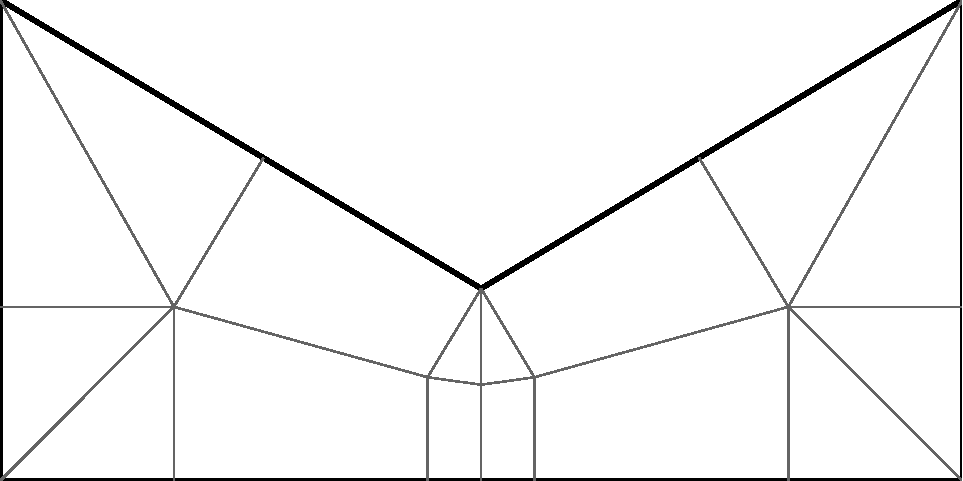
\includegraphics[width=.3\linewidth,rotate=-90]{response_simple_example_1}
\includegraphics[width=.3\linewidth,rotate=-90]{response_simple_example_2}
\includegraphics[width=.3\linewidth,rotate=-90]{response_simple_example_3}
\caption{Skeletal trapezoidation}\label{overview_outline}
\end{figure}






\Que{
As the authors correctly point out, the MA is not piecewise linear even for polygonal boundaries. In 3.2, second paragraph, the authors state that "the medial axis is a compact and complete representation of the shape". First, the MA + the radius function can be considered a shape representation, which is not true for the MA by itself. Second, the statement that the authors is meant to be generic, but it is not clear what compact means for a medial axis that is not piecewise linear. One can argue that the polygon itself is a rather compact representation of the shapes considered in this manuscript. 
}
\Ans{
Indeed the statement was meant generically, but we agree it lacked substance.
The wording is now changed to better describe the general role of the medial axis in research.
}
\commits{d3f19c04e3bb0d80c0b162531dbf576fc705d77c}
\paper{Medial axis transform}{
The medial axis is a \revise{compact and complete representation of}{representation commonly used to analyse} a shape.
}




\Que{
More generally, the technique seems to effectively be a variable offset scheme, but there is little discussion about what is known about variable offsets. 
Find more literature
}

\todo{
elber1991error, 
}





\Que{
Moreover, the proposed technique seems to rely on rather accurate control of the width w of the deposited material, but it is not clear whether such control is achievable in practice. 
}
\Ans{
The photos of our print results already showed that adaptive width control is possible up to some (admittedly insufficient) extent.
We have developed a new method for actualizing adaptive width control which can readily be applied to unmodified FDM systems such as the Ultimaker S5: linear backpressure compensation.
We show the results of linear backpressure compensation in a separate figure which clearly shows the achieved variance in bead width.
}
\todo{
Show S5 prints. 
The proposed technique relies \emph{less} on the accuracy of the control than existing techniques – as exemplified by Fig 17b.
}
\commits{3d7238e2787f17c4cff63804eb4b84439ff85f1b }
\paper{5.2 Printing results}{
\revise{}{
Test prints were performed on an unmodified Ultimaker S5 system,
with a standard  \SI{0.4}{\milli\meter} nozzle
and PLA filament
and a layer thickness of $h=\SI{0.1}{\milli\meter}$.
In order to accurately realize a varying bead width we vary the movement speed, while keeping the internal pressure in the system constant.
One approach would be keep the filament inflow $f$ (in \si{\milli\meter\cubed\per\second}) constant by varying movement speed accordingly.
However, that doesn't result in the intended filament outflow variation - see \cref{zero_backpressure}.
We conjecture that the filament outflow is related to the total pressure in the system,
which depends not only on the amount of filament in between the feeder wheel and the nozzle (which we keep constant), 
but also depends on the backpressure that the previous layer exerts on the filament protruding from the nozzle.
We conjecture that the amount of backpressure is monotonically related to the requested line width and compensate for the backpressure using a simple linear model:

\begin{align}
 v(w) &= \frac{f(w)}{h w} \\ 
% f &\sim p \\
% p &= p_\text{in} + p_\text{ext} \\
% p_\text{in} &= C \\
% p_\text{ext} &\sim w \\
% p_\text{ext} &= w / w^* - 1 \\
% f &= f^* - k p_\text{ext} \\
 f(w) &= f_0 - k \left( w / w_0 - 1 \right) \\
 f_0 &= v_0 w_0 h 
% v &= \frac{f^* - k p_\text{ext}}{h w} \\ 
% v &= \frac{v^* w^* h - k (w / w^* - 1)}{h w}
\end{align}
where
$v(w)$ is the movement speed as a function of requested bead width $w$,
$f(w)$ is the filament outflow,
$f_0$ is a constant reference flow
and
$k$ is the amount of backpressure compensation.
Using increments of $0.1$ we established that using a factor of $k=1.1$ yields satisfactory bead width variation for our setup where
$v_0=\SI{30}{\milli\meter\per\second}$, 
$w_0=\SI{0.4}{\milli\meter}$.
See \cref{backpressure}.

\begin{figure}
\centering
\setlength{\figwidth}{0.32\columnwidth}
\setlength{\figheight}{0.5\columnwidth}
\begin{subfigure}[t]{\figwidth}\centering
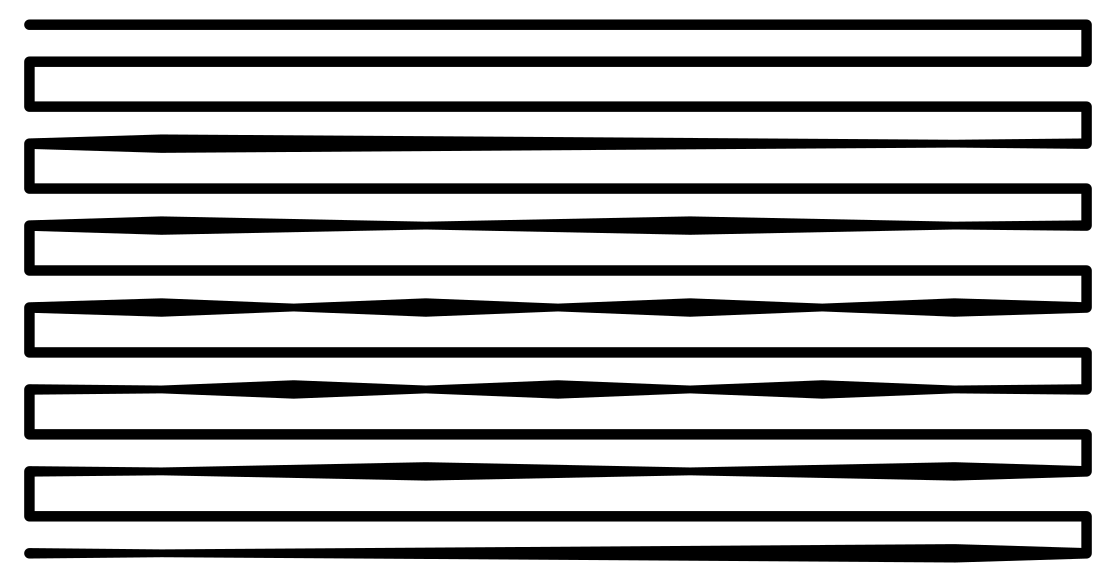
\includegraphics[angle=90,height=\figheight]{sources-validation-backpressure-compensation-target.pdf}
\caption{Target widths}\label{backpressure_target}
\end{subfigure}
\begin{subfigure}[t]{\figwidth}\centering
\includegraphics[angle=90,height=\figheight]{sources-validation-zero-backpressure-compensation.png}
\caption{Constant filament inflow (\si{\milli\meter\cubed\per\second})}\label{zero_backpressure}
\end{subfigure}
\begin{subfigure}[t]{\figwidth}\centering
\includegraphics[angle=90,height=\figheight]{sources-validation-backpressure-compensation.png}
\caption{Backpressure compensation}\label{backpressure}
\end{subfigure}
\caption{
Print results of varying width test on top of a dense white raft.
Trying to reproduce \subref{backpressure_target} without backpressure compensation ($k=0$) yields worse results \subref{zero_backpressure} than with backpressure compensation $k=1.1$ \subref{backpressure}.
}
\label{backpressure_compensation}
\end{figure}

}
}




\Que{
At the same time, the scheme can potentially result in trajectories with many inflection points - this is slow and demanding for the machine. 
}
\Ans{
We have added statistics on fabrication time and discussed our findings.
See our response to 1.3.
}





\Que{
Finally, the examples provided depict the results obtained by the authors by "emulating" other techniques, but not with the actual results produced by the other techniques. While the reason behind this choice is easy to guess, it weakens the effectiveness of the claims. Adding careful discussions/extensions to support these questions would make the paper stronger.
}
\todo{
Discuss how much the over-fill / underfill and bead width variation depend on the fact that our reimplementations are only approximations.
}








\section{Reviewer 3}
Paper is well written. It is mostly easy to follow but overall, I find the the contributions somewhat incremental and the motivation not convincing. The paper mostly feels like a technical report. I am not sure if the methods overall teach enough to the researchers in the field to open up new research possibilities. My specific comments are below: 





\Que{
The title is a little misleading that the presented approach may be used for general “Additive Manufacturing”. However, my understanding from the text is that it is designed particularly for FDM. I believe it is important to highlight this in the title. Otherwise, there should be enough evidence to prove that it can be applied to other kinds of printing processes, such as SLS, SLA, DMLS etc. 
}
The title has changed.
\revise{additive manufacturing}{fused deposition modeling}
\commits{64eb2f2c1cbb28258a984b5f84ea6e3a039ee1f0}
\paper{Title}{
A framework for adaptive width control of dense contour-parallel toolpaths in \revise{additive manufacturing}{fused deposition modeling}
}





\Que{
It would be nice to discuss why contour-parallel toolpaths are needed or selected. In what situations, these are required as opposed to zigzag style (or direction-parallel as referred in the text) patterns. Without such a discussion, the motivation seems a little weak. In the second paragraph of introduction, there is a short discussion about this but it sounds like the authors assume that even the perimeters (or outline) are printed with direction-parallel extrusion. However, common approach in FDM is to print the perimeters with contour parallel toolpaths and fill the inner region with direction-parallel paths only (as later acknowledged in the related work 3rd paragraph). I think the motivation for contour parallel toolpaths needs to be justified further. 
}
\Ans{
The industry standard is to use a combination of contour-parallel and direction-parallel.
We now clarify why contour-parallel is (partly) used and that in as much as contour-parallel is used, our approach improves on the industry standard.
We have also developed and presented a new meta-scheme for generating only a limited number of perimeters, which shows that our technique is compatible with the industry standard for FDM 3D printing.
}

\commits{6b0f8c78d31bd0c6946885da96f73f1cfc1a21ae ac800628951417dcb28bd6e3a0ed08801735acf4 a88ccd3309aef1233ed00ce9f22b244fe64668f4 077c8ee138bb311a8ba9abf303af4b09e973637a}
\paper{Intro}{
\revise{
Contour-parallel extrusion therefore leads to a less bumpy outline shape than direction-parallel extrusion does.
}{
Because contour-parallel extrusion leads to a more accurate outline shape it is common practice to print either the whole layer or only a limited number of outer perimeters that way.
This paper improves on those contour-parallel toolpaths and addresses several issues which commonly occur in 3D models with narrow geometry.
}
}
\paper{Abstract}{
\revise{By densely filling consecutive 2D layers with contour-parallel extrusion toolpaths, FDM can produce parts with high stiffness and strength.}
{High stiffness parts are produced by filling the 2D polygons of consecutive layers (partly) with contour-parallel extrusion toolpaths.}
}




\Que{
Related work acknowledges the previous work sufficiently. However, the differences between the state of the art and the presented work are not clear. More discussion on where this work stands with respect to the state of the art is required. 
}
\Ans{
We have tried to address this in response to several other reviewers' comments.
See our response to 1.5, 1.1.1.
We now clearly claim that our method produces a lower range of bead widths than the state-of-the-art.
}
\todo{link with other responses}
\commits{004894210fbc961f82b792fc702d1b67a1a8e8e8}
\paper{Fig 1}{
\subref{intro_wedge_distributed} Our approach minimizes over- and underfill with \revise{beads close to the nozzle size}{less extreme widths}.
}






\Que{
Isn’t it possible to put bounds on the width in the existing methods, such as the approach described in [9]? More discussion on that would be helpful. 
}
\Ans{
The bead width in Jin et al. is limited to $0.5 w^*$ to $1.8 w^*$ , which means the variation is a factor of $3.2$;
this was already described in the related work section, but the factor was wrongly said to be $2$ instead of $3.2$.
We emphasized that our method (generally) results in a bead width deviation of $2$, rather than $3.2$ in the related work section and in the discussion section.
}
\commits{661d8f6766548c287cb174070432097e396d198f 92217c04e118dcf6f65b16a1ffcdfa40b4d50c0d}
\paper{Intro}{
The current state-of-the-art for FDM printing developed by \citeauthor{Jin2017JMS} employs a strategy which alters the widths of the centermost beads at most by a factor of \revise{$2$}{$3.2$}~\cite{Jin2017JMS},
}
\paper{Discussion}{
In \cref{TEST_Center_accuracy} we can see that
the centered beading scheme effectively deals with both overfill and underfill and produces desired bead widths in all locations, except for the extrusion paths in the center, where the bead widths \revise{are within a factor 2 off from the desired bead width.}{range between $0.5 w^*$ and $1.8w^*$, i.e. the deviation is within a factor of $3.2$.}
}
\paper{Discussion}{
\revise{}{Moreover, because the quantization operator rounds to the nearest number of beads the bead widths range from $0.75w^*$ to $1.5w^*$, i.e. the deviation is within a factor $2$, which is considerably lower than in the centered scheme.}
We therefore conclude that the distributed schemes \revise{result in bead widths closer to the preferred widths}{exhibit a lower bead width deviation} compared to the centered scheme.
}



\Que{
Figure 4 and corresponding explanation in Section 3.2 are confusing. Why such decomposition is needed is not clear to me. 
}
\todo{
Maybe put something like “this figure is for back-reference if you forgot what a thing is for”

Are you sure you mean figure 4? Maybe figure 3 or figure 2?
}





\Que{
In Figure 3, why some of the edges in (c) (the ones in the center area) disappear in (d)?
}
\Ans{
Fixed. Fig 3 c and d now have the same discretization.
}
\commits{43cadb352a6a276bbaaab53f9b5b217bec4b3a2e}





\Que{
It is unclear how some of the parameters are adjusted, such as $\alpha_\text{max}, d_\text{max}^\text{unmarked}, d_\text{transition}^\text{max}, t_\text{beading}, d_\text{intersection}^\text{max}$. What are their effects on the end result? Selections seem somewhat arbitrary. 
}
\todo{
Make my reasons for choosing these more explicit
}






\Que{
Is this approach generalizable to sparse infill? It is very common in FDM to use a sparse infill and only use dense fill on surface regions.
}
\Ans{
The goal of sparse infill on the otherhand is to generate intentional spacing between lines; this is not reconcilable with the goal of preventing underfill.
However, we did show that the contour-parallel toolpaths can be combined with sparse infill.
See our response to 3.2.
}






\Que{
If this is used for outer surface, what are the implications on the surface quality in comparison to other approaches? 
}
\todo{
This is one of the usecases why this is a good method
Discuss effect of this algorithm on the outline accuracy
}





\Que{
I think Figure 13 should be replaced with a table. 
}
\Ans{
Indeed. Done.
}
\commits{735762b1e7daf31ae4465bf288ef867ded7da095}
% commit only now shows table




\Que{
In text, some references are missing, such as first sentence of “Outer bead” paragraph in Section 4 (Moesen et al [?]), first sentence of “Constant bead count” (Ding et al [?]) paragraph in Section 4 etc. 
}
\Ans{
We cannot reproduce this typesetting bug. Please inform the proofing department to take extra care of these references when preparing this manuscript for publication.
}





\Que{
Evaluation in the results section is overall good but it is not clear what are the implications of the presented approach on the complete 3D result. A discussion on this would be helpful.
}
\todo{
Perhaps discuss effect of width changes on amount of fusing between layers
}





\Que{
What are the limitations of the presented algorithm? I do not see any discussions of the limitations of the algorithm.
}
\todo{
Linear approximations 

a lot of direction changes (?)
}













\section{Other changes}
We have fixed some issues with positions and colors being swapped in the statistical analysis subfigures.
Fig 17f colors are adjusted.
Fig 17e and 17f are swapped.
\commits{43cadb352a6a276bbaaab53f9b5b217bec4b3a2e}

Improvements to abstract.
\commits{c5ecf8f8c5c15266059278a6b4c26774446e7854}
\paper{Abstract}{
Toolpath with uniform inward offsets from the outline polygons produce over- and underfill regions in the center of the shape, which are especially problematic for thin parts such as casings and microstructures.
\revise{Toolpath with uniform }{Toolpaths consisting of \emph{uniform}} inward offsets from the outline polygons produce over- and underfill regions in the center of the shape, which are especially \revise{problematic for }{detrimental to the mechanical performance of} thin parts such as casings and microstructures.
 Existing approaches for generating toolpaths with adaptive width result in a large variation in widths, which for some hardware systems is difficult to realize accurately, if not beyond their capabilities.
 In this paper we present a framework which supports multiple schemes to generate toolpaths with adaptive width, by using a function to decide the number of beads and their widths which are applied from the center outward.
Furthermore, we propose a novel scheme for FDM printing which \revise{avoids}{reduces} extreme bead width deviation\revise{ from the nozzle size}{}, \revise{and limits}{while limiting} the number of altered toolpaths.
We validate the effectiveness of our framework and this novel scheme on a data set of 300 \revise{slices}{layer outlines}.
}



Fix double header of References.
\commits{7597b176f6a88ae98c8c7a4c791475af356b3da6}

Added patent notice and url to open source implementation.
\commits{ff3c09037f05eba5028cb51bf8cd6c0bb77a0b0a}
\paper{Intro}{
\revise{}{The presented framework is patented by Ultimaker and open source available at \url{github.com/Ultimaker/libArachne}.}
}

Lil
\commits{5f5c4c640d94010816e6d6d5934a2dc016b4d172}



\end{document}
